\documentclass{article}
\usepackage[utf8]{inputenc}
\usepackage{color}
\usepackage{graphicx}
\usepackage{amsmath}
%Here are TA pre-defined

\newcommand{\DC}{Dr. Da-Cheng Juan}
%The following are some notation you may use
\newcommand{\Asca}{$\mathit{a}$}
%A scalar (integer or real)
\newcommand{\Avec}{$\bm{a}$}
%A vector
\newcommand{\Amatrix}{$\bm{A}$}
%A matrix
\newcommand{\Atensor}{\textsf{A}}
%A tensor
\newcommand{\nIM}{$I_n$}
%Identity matrix with n rows and n columns
\newcommand{\IM}{$I$}
%Identity matrix with dimensionality implied by context
\newcommand{\StaBasisVec}{$e^{(i)}$}
%Standard basis vector [0,...,0,1,0,...,0] with a 1 at position i
\newcommand{\diagA}{$diag(a)$}
%A square, diagonal matrix with diagonal entries given by a
\newcommand{\Ascarand}{\texttt{a}}
%A scalar random variable
\newcommand{\Avecrandom}{\texttt{\textbf{a}}}
%A vector-valued random variable
\newcommand{\Amatrixrandom}{\texttt{\textbf{A}}}
%A matrix-valued random variable
\newcommand{\Aset}{$\mathbb{A}$}
%A set
\newcommand{\realNumSet}{$\mathbb{R}$}
%The set of real numbers
\newcommand{\setZeroOne}{$\mathit{\{0,1\}}$}
%The set containing 0 and 1
\newcommand{\setN}{$\mathit{\{0,1,...,n\}}$}
%The set containing 0 and 1
\newcommand{\intervalAB}{$\mathit{[a,b]}$}
%The real interval including a and b
\newcommand{\intervalexcAB}{$\mathit{(a,b]}$}
%The real interval excluding a but including b
\newcommand{\setSub}{$\mathbb{A}$ \textbackslash $\mathbb{B}$}
%Set subtraction, i.e., the set containing the  elements of A that are nit in B
\newcommand{\graph}{$\mathcal{G}$}
%A graph
\newcommand{\parentG}{$\mathit{Pa_\mathcal{G} (X_i)}$}
%The parents of xi in G
\newcommand{\elemiofveca}{$\mathit{a_i}$}
%Element i of vector a, with indexing starting at 1
\newcommand{\allelemofvecaexi}{$\mathit{a_{-i}}$}
%All elements of vector a except for element i
\newcommand{\matrixij}{$\mathit{A_{i,j}}$}
%Element i,j of matrix A
\newcommand{\rowi}{$\mathit{A_{i,:}}$}
%Row i of matrix A
\newcommand{\columni}{$\mathit{A_{:,i}}$}
%Column i of matrix A
\newcommand{\tensorijk}{$\mathrm{A_{\mathit{i},\mathit{j},\mathit{k}}}$}
%Element (i,j,k) of a 3-D tensor A
\newcommand{\twodenoftensor}{$\mathrm{A_{:,:,\mathit{i}}}$}
%2-D slice of a 3-D tensor
\newcommand{\randveci}{$\mathrm{a_{\mathit{i}}}$}
%Element i of the random vector a
\newcommand{\transA}{$\mathit{A^{\top}}$}
%Transpose of matrix A
\newcommand{\pesudoinverseA}{$\mathit{A^+}$}
%Moore-Pen-rose pseudo-inverse of A
\newcommand{\prductAB}{$\mathit{A \odot B}$}
%Element-wise (Hadamard) product of A and B
\newcommand{\detA}{$\mathit{det(A)}$}
%Determinant of A
\newcommand{\derivative}{$\frac{\mathrm{d}y}{\mathrm{d}x}$}
%Derivative of y with respect to x
\newcommand{\partialDerivative}{$\frac{\mathrm{\partial}y}{\mathrm{\partial}x}$}
%Partial derivative of y with respect to x
\newcommand{\gradient}{$\nabla_{\mathit{x}} \mathrm{y}$}
%Gradient of y with respect to x
\newcommand{\matrixDeriative}{$\nabla \mathrm{x} \mathrm{y}$}
%Matrix derivative of y with respect to X
\newcommand{\tensoeDeriative}{$\nabla \textsf{x} \mathrm{y}$}
%Tensor containing derivative of y with respect to X
\newcommand{\jacobianMatrix}{$\frac{\mathrm{\partial}f}{\mathrm{\partial}x}$}
%Jacobian matrix J ∈ R^(m*n) of f: R^n → R^m 
\newcommand{\hessianMatrix}{$\nabla_{\mathit{x}}^2 f(\mathit{x})$ or $\mathbf{H}(\mathit{f})(\mathit{x})$}
%The Hessian matrix of f at input point x
\newcommand{\intOverDomainX}{$\int {f(\mathit{x}) \mathrm{d}x}$}
%Define integer over the entire domain of x
\newcommand{\intOverSetS}{$\int_\mathbb{S} {f(\mathit{x}) \mathrm{d}x}$}
%Define integer with respect to x over the set S
\newcommand{\independantAB}{$a \perp b$}
%The random variables a and b are independent
\newcommand{\independantABGivenC}{$a \perp b \mid c$}
%They are conditionally independent given c
\newcommand{\probability}{$P(a)$}
%A probability distribution over a discrete variables
\newcommand{\probabiltyOverContinuousVariables}{$p(a)$}
%A probability distribution over a continuous variable, or over a variable whose type has not been specified
\newcommand{\randomVariable}{$a \sim P$}
%Random variable a has distribution P
\newcommand{\expectation}{${\mathbb{E}}_{x \sim P}[f(\mathit{x})]$ or $\mathbb{E}f(\mathit{x})$}
%Expectation of f(x) with respect to P(x)
\newcommand{\variance}{$\mathrm{Var}(f(\mathit{x}))$}
%Variance of f(x) under P(x)
\newcommand{\covariance}{$\mathrm{Cov}(f(\mathit{x}),g(\mathit{x}))$}
%Covariance of f(x) and g(x) under P(x)
\newcommand{\shannon}{$H(x)$}
%Shannon entropy of the random variable x
\newcommand{\kullbackleibler}{$D_{KL}(P \parallel Q)$}
%Kullback-Leibler divergence of P and Q
\newcommand{\gaussian}{$\mathcal{N}(\mathit{x},\mu, \Sigma)$}
%Gaussian distribution over x with mean μ and covariance Σ
\newcommand{\functionAtoB}{$f : \mathbb{A} \to \mathbb{B}$}
%The function f with domain A and range B
\newcommand{\compositionFG}{$f \circ g$}
%Composition of the function f and g
\newcommand{\parametrized}{$f(\mathit{x} ; \theta)$}
%A function of x parametrized by θ. (Sometimes we write f(x) and omit the argument θ to lighten notation)
\newcommand{\logx}{$\mathrm{log} \mathit{x}$}
%Natural logarithm of x
\newcommand{\sigmoid}{$\sigma (\mathit{x})$}
%Logistic sigmoid, 1/(1 + exp(-x))
\newcommand{\softplus}{$\zeta(\mathit{x})$}
%Soft-plus, log(1 + exp(x))
\newcommand{\pnorm}{$\| \mathit{x} {\|}_{\mathit{p}}$}
%L^p norm of x
\newcommand{\twonorm}{$\| \mathit{x} \|$}
%L^2 norm of x
\newcommand{\positivepart}{${\mathit{x}}^+$}
%Positive part of x, i.e., max(0,x)
\newcommand{\condition}{$1_{condition}$}
%is 1 if the condition is true, 0 otherwise
\newcommand{\dataGneeratingP}{${\mathit{P}}_{\mathrm{data}}$}
%The data generating distribution
\newcommand{\pDefinedByTrainingSet}{${\hat{\mathit{P}}}_{data}$}
%The empirical distribution defined by the training set
\newcommand{\trainingEx}{$\mathbb{X}$}
%The set of training examples
\newcommand{\ithEx}{$\mathit{x}^{(\mathit{i})}$}
%The i-th example (input) from a dataset
\newcommand{\targetforSL}{${\mathit{y}}^{(\mathit{i})}$ or ${\bm{\mathit{y}}}^{(\mathit{i})}$}
%The target associated with x^(i) for supervised learning
\newcommand{\inputEx}{$\mathbf{X}$}
%The m*n matrix with input example x^(i) in row X_(i,:)

%Ch2.1 
%Ch3.1

\begin{document}
\title{Class Note}
\Large{Course: Machine Learning}

\Large{Lecturer: Dr. Da-Cheng Juan}
\section{ReadMe}
\label{ReadMe}
main.tex is the main file, outlining all the section. Please take your lecture note into Ch\ref{Ch2.1} 

Change word size \tiny{Hi} \Huge{Hi} \Large{Hi}

Change word color \textcolor{red}{Hi} \textcolor{blue}{Hi}

Italic:\textit{Hi} 

Bold:\textbf{Hi} 

Put a pic here
\begin{figure}[htb]
\centering
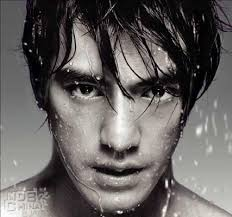
\includegraphics[width=0.5\textwidth]{FIG/mypic.jpg}
\caption{This is me} 
\label{mypic}
\end{figure}

Fig.\ref{mypic} is my picture.

We define some commands in dft.tex, before you type a new label, please check it is already exist or not. For example, Dr. Da-Cheng Juan is \DC. You can add your new command into dft.tex, but also add comment and used in which chapter. 

Math inline mode:\\
A polynomial: $x^{3} + 2x^{2} + x$\\
A series: $a_{1}, a_{2}, a_{3}, a_{4}, a_{5}$\\
$x^{2y^{3}}$ $x^{2y_{2}}$ $x^{y}_{1}$ $x_{1}^{y}$\\

Math display mode:\\
\[
\sum_{i=1}^{n}{n^2-3n+4} = f(n)
\]
\begin{equation}
\label{myequation}
\sum_{i=1}^{n}{n^2-3n+4} = f(n)
\end{equation}


\section{Ch2.7 Eigendecomposition}
\label{Ch2.7}

Eigendecomposition is a method that try to decompose matrix into several simple parts,
  eigenvectors and eigenvalues.

\begin{itemize}
  \item Eigenvector and Eigenvalue

  % eq 2.39
  \begin{equation} \tag{2.39}
    \label{eq_2_39}
    \bm{Av} = \lambda \bm{v}
  \end{equation}

  Try to find a vector $\bm{v}$ that $\bm{Av}$ is the scale of $\bm{v}$.
    The scaler $\lambda$ is the eigenvalue that corresponding to this eigenvector.
    The eigenvector is still eigenvector after scaling.

  \item Eigendecomposition

  Concatenate all the eigenvectors $\bm{v} ^ {(1)} , \ldots , \bm{v} ^ {(n)}$
    and corresponding eigenvalues $\lambda _ {1} , \ldots , \lambda _ {n}$
    into matrix $\bm{V} = [ \bm{v} ^ {(1)} , \ldots , \bm{v} ^ {(n)} ]$
    and vector ${\bm{\lambda} = [ \lambda _ {1} , \ldots , \lambda _ {n} ]} ^ \top$
    respectively.

  We could say that the matrix $\bm{A}$ could be decomposed into matrix $\bm{V}$ and vector $\bm{\lambda}$ by:

  % eq 2.40
  \begin{equation} \tag{2.40}
    \label{eq_2_40}
    \bm{A} = \bm{V} diag(\bm{\lambda}) \bm{V} ^ {-1}
  \end{equation}

  \newpage

  \item Real Symmetric Matrix Eigendecomposition

  % fig 2.3
  \setcounter{figure}{2}
  \begin{figure}[ht]
    \begin{center}
      Effect of eigenvectors and eigen values\par
      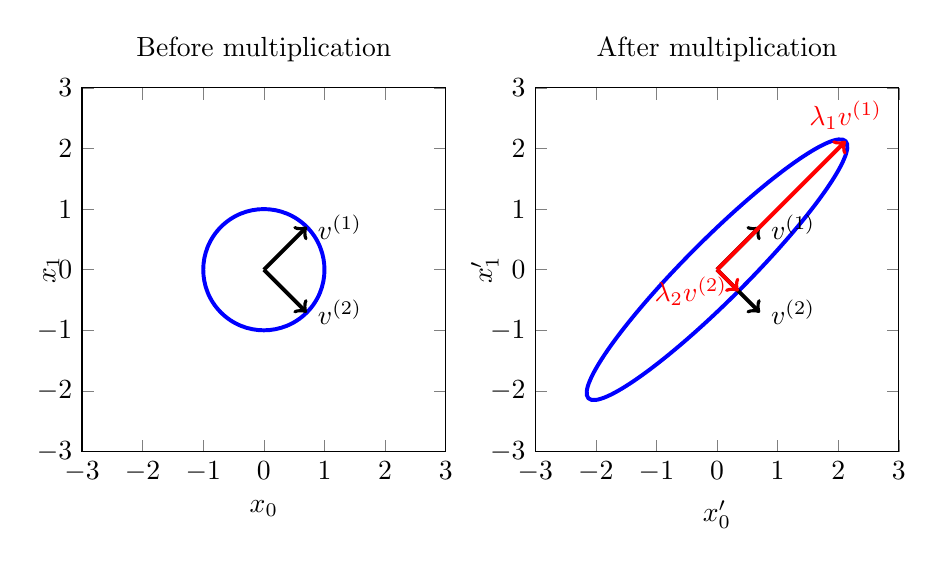
\begin{tikzpicture}[
          scale=1,
        ]
        \begin{axis}[
          name = plot1,
          width=6.2cm,
          height=6.2cm,
          trim left,
          xmin = -3,
          xmax = 3,
          ymin = -3,
          ymax = 3,
          xlabel = $x_0$,
          xtick = {-3, -2, -1, 0, 1, 2, 3},
          ylabel = $x_1$,
          ylabel style = {yshift=-1.5em},
          ytick = {-3, -2, -1, 0, 1, 2, 3},
          title = {Before multiplication},
        ]
          \draw [blue, line width=0.5mm] \pgfextra{
            \pgfpathellipse{
              \pgfplotspointaxisxy{0}{0}
            }
            {\pgfplotspointaxisdirectionxy{cos(45)}{sin(45)}}
            {\pgfplotspointaxisdirectionxy{cos(315)}{sin(315)}}
          };
          \draw [->, line width=0.5mm] (axis cs:0,0) node {} -- (axis cs:{cos(45)},{sin(45)}) node[right] {$v ^ {(1)}$};
          \draw [->, line width=0.5mm] (axis cs:0,0) node {} -- (axis cs:{cos(315)},{sin(315)}) node[right] {$v ^ {(2)}$};
        \end{axis}


        \begin{axis}[
          name = plot2,
          at = (plot1.right of south east),
          anchor = left of south west,
          width=6.2cm,
          height=6.2cm,
          trim left,
          xmin = -3,
          xmax = 3,
          ymin = -3,
          ymax = 3,
          xlabel = $x_0'$,
          xtick = {-3, -2, -1, 0, 1, 2, 3},
          ylabel = $x_1'$,
          ylabel style = {yshift=-1em},
          ytick = {-3, -2, -1, 0, 1, 2, 3},
          title = {After multiplication},
        ]
          \draw [blue, line width=0.5mm] \pgfextra{
            \pgfpathellipse{
                \pgfplotspointaxisxy{0}{0}
            }
            {\pgfplotspointaxisdirectionxy{3*cos(45)}{3*sin(45)}}
            {\pgfplotspointaxisdirectionxy{.5*cos(315)}{.5*sin(315)}}
          };
          \draw [->, line width=0.5mm] (axis cs:0,0) node {} -- (axis cs:{cos(45)},{sin(45)}) node[right] {$v ^ {(1)}$};
          \draw [->, line width=0.5mm] (axis cs:0,0) node {} -- (axis cs:{cos(315)},{sin(315)}) node[right] {$v ^ {(2)}$};
          \draw [->, red, line width=0.5mm] (axis cs:0,0) node {} -- (axis cs:{3*cos(45)},{3*sin(45)}) node[above] {$\lambda _ 1 v ^ {(1)}$};
          \draw [->, red, line width=0.5mm] (axis cs:0,0) node {} -- (axis cs:{.5*cos(315)},{.5*sin(315)}) node[left] {$\lambda _ 2 v ^ {(2)}$};
        \end{axis}

      \end{tikzpicture}
      \caption{Effect of eigenvectors and eigenvalues. An example of the effect of eigenvectors and eigenvalues. Here, we have a matrix $\bm{A}$ with two orthonormal eigenvectors, $\bm{v} ^ {(1)}$ with eigenvalue $\lambda _ 1$ and $\bm{v} ^ {(2)}$ with eigenvalue $\lambda _ 2$. \textit{(Left)} We plot the set of all unit vectors $\bm{u} \in {\mathbb{R}} ^ 2$ as a unit circle. \textit{(Right)} We plot the set of all points $\bm{Au}$. By observing the way that $\bm{A}$ distorts the unit circle, we can see that it scales space in direction $\bm{v} ^ {(i)}$ by $\lambda _ i$}
      \label{fig:effect_of_eigenvectors_and_eigen_values}
    \end{center}
  \end{figure}

  % eq 2.41
  \begin{equation} \tag{2.41}
    \label{eq_2_41}
    \bm{A} = \bm{Q} \bm{\Lambda} \bm{Q} ^ \top
  \end{equation}

  % TODO: Ch 2.7 page 42
  \eqref{eq_2_41} is derided from \eqref{eq_2_40}.
  $\bm{Q}$ is an orthogonal matrix composed of eigenvectors of $\bm{A}$
  , and $\bm{\Lambda}$ is a diagonal matrix which $\Lambda _ {i,i}$ is associated with the eigenvector in column $i$ of $\bm{Q}$.
  Figure~\ref{fig:effect_of_eigenvectors_and_eigen_values} for the example.

  \newpage

  \item Eigendecomposition Characteristics

  \begin{itemize}

    \item Singular

    matrix is singular $\iff \forall \lambda = 0$

    \item Quadratic Expression Optimization

    if ${\| \bm{x} \|} _ 2 = 1,\ f(\bm{x}) = \bm{x} ^ \top \bm{A} \bm{x}$ is optimal.
    $\bm{x}$ is an eigenvector of $\bm{A}$, the $max(f(\bm{x}))$ is maximum eigenvalue, the $min(f(\bm{x}))$ is minimum eigenvalue.

    \item Positive Definite, Positive Semidefinite, Negative Definite, and Negative Semidefinite
    \begin{itemize}
      \item Positive Definite: $\forall \lambda > 0$

        Extra Characteristics: $\bm{x} ^ \top \bm{A} \bm{x} = 0 \Rightarrow \bm{x} = 0$

      \item Positive Semidefinite: $\forall \lambda \geq 0$

        Extra Characteristics: $\forall \bm{x}, \bm{x} ^ \top \bm{A} \bm{x} \geq 0$

      \item Negative Definite: $\forall \lambda < 0$
      \item Negative Semidefinite: $\forall \lambda \leq 0$
    \end{itemize}

  \end{itemize}

\end{itemize}


\section{Ch6.2 Gradient-Based Learning}
\label{Ch6.2}
% 1p

\subsubsection{Cost Function}
% 0.5P
To build the cost function, we use the cross-entropy between the training data and the model’s predictions. The total cost function combine the primary cost function with a regularization term.

\subsubsubsection{Learning Conditional Distributions with Maximum Likelihood}
% 1.25p
Cost function is the negative log-likelihood, equivalently described as the cross-entropy between the training data and the model distribution.

  % eq 6.12
  \begin{equation} \tag{6.12}
   \label{eq_6_12}
    J( \bm{\theta} ) = - \mathbb{E} _ {\bm{\mathrm{x}}, \bm{\mathrm{y}} \sim \hat{p} _ \mathrm{data} } 
          \log p _ \mathrm{model} ( \bm{y}\ |\ \bm{x} )
  \end{equation}

The cost function changes depending on the specific form of $logp_{model}$.
if $p_{model}(\bm{y}\  |\ \bm{x})=\mathcal{N}(\bm{y};\mathit{f}(\bm{x};\theta),\bm{I})$

  % eq 6.13
  \begin{equation} \tag{6.13}
   \label{eq_6_13}
    J( \theta ) = \frac{1}{2} \mathbb{E} _ {\bm{\mathrm{x}}, \bm{\mathrm{y}} \sim \hat{p}_ \mathrm{data}}
        \| \bm{y} - f( \bm{x} ; \bm{\theta} ) \| ^ 2 + \mathrm{const}
  \end{equation}

\subsubsubsection{Learning Conditional Statistics}
% 1.25p
Using calculus of variations to solve the optimization problem.
First result:

  % eq 6.14
  \begin{equation} \tag{6.14}
   \label{eq_6_14}
   f ^ * = {\arg \min} _ {f} \mathbb{E} _ {\bm{\mathrm{x}}, \bm{\mathrm{y}} \sim p _ \mathrm{data}} 
       \| \bm{y} - f( \bm{x} ) \| ^ 2
  \end{equation}
  
  % eq 6.15
  \begin{equation} \tag{6.15}
   \label{eq_6_15}
    f ^ * (\bm{x}) = \mathbb{E} _ {\bm{\mathrm{y}} \sim p _ \mathrm{data} ( \bm{y} | \bm{x} ) } [ \bm{y} ]
  \end{equation}
  
Second result:

  % eq 6.16
  \begin{equation} \tag{6.16}
   \label{eq_6_16}
   f ^ * = {\arg \min} _ {f} \mathbb{E} _ {\bm{\mathrm{x}}, \bm{\mathrm{y}} \sim p _ \mathrm{data}} 
       \| \bm{y} - f( \bm{x} ) \| _ 1
%   \mathit{f}^*=\arg\min_{\mathit{f}}\ \mathbb{E}_{x,y\sim\mathit{p}_{data}}\|\bm{y}\ -\ \mathit{f}(\bm{x})\|_1
  \end{equation}

\subsubsection{Output Units}
% 0.5p
$\bm{h} = f( \bm{x}; \bm{\theta})$ defines a set of hidden features which is provided by the feedforward network.

\subsubsubsection{Linear Units for Gaussian Output Distributions}
% 0.5p
Linear output units produces a vector $\hat{\bm{y}} = \bm{W} ^ \top \bm{h} + \bm{b}$
Using Linear output layers to produce the mean of a conditional Gaussian distribution:

  % eq 6.17
  \begin{equation} \tag{6.17}
   \label{eq_6_17}
   p(\bm{y}\ |\ \bm{x}) = \mathcal{N}(\bm{y}; \hat{\bm{y}}, \bm{I})
  \end{equation}

\subsubsubsection{Sigmoid Units for Bernoulli Output Distributions}
% 2.25p
The neural net needs to predict only $P(y=1\ |\ \bm{x})$ in a Bernoulli distribution.
We use a linear unit and threshold its value to get a valid probability.

  % eq 6.18
  \begin{equation} \tag{6.18}
   \label{eq_6_18}
   P(y = 1\ |\ \bm{x}) = \max \{ 0, \min \{ 1, \bm{w} ^ \top \bm{h} + b \} \}
  \end{equation}
  
A sigmoid output unit:

  % eq 6.19
  \begin{equation} \tag{6.19}
    \label{eq_6_19}
    \hat{y} = \sigma( \bm{w} ^ \top \bm{h} + b)
  \end{equation}
  
Normalize to see this yields a Bernoulli distribution controlled by a sigmoidal transformation of z:

  % eq 6.20 ~ 6.23
  \setcounter{equation}{20}
  \begin{align} \tag{6.20}
   \label{eq_6_20}
    \log \tilde{P}(y)& =yz\\
    \tilde{P}(y)& = \exp(yz)\\
    P(y)& =\frac{\exp(yz)}{\sum _ {y'=0} ^ {1} \exp(y'z) }\\
    P(y)& =\sigma( (2y-1)z )
  \end{align}
  
The loss function for maximum likelihood learning of a Bernoulli parametrized by a sigmoid:

  % eq 6.24 ~ 6.26
  \setcounter{equation}{24}
  \begin{align} \tag{6.24}
   \label{eq_6_24}
    J(\bm{\theta})& = - \log P(y\ |\ \bm{x})\\
    & = - \log \sigma( (2y-1)z )\\
    & = \zeta( (1-2y)z )
  \end{align}

  \subsubsubsection{Softmax Units for Multinoulli Output Distributions}
  % 3.25p
  Softmax functions are often used as a classifier, to classified $n$ different classes.

  We want to generalize the Bernoulli distribution to multinoulli distribution.

  % eq 6.27
  \begin{equation} \tag{6.27}
    \label{eq_6_27}
    \hat{y} = P( y=1\ |\ \bm{x} )
  \end{equation}

  The~\eqref{eq_6_27} shows a example of maximum likelihood defined by Bernoulli distribution.
  Next, using log-likelihood to simplify computation. We take $z _ i = \log \tilde{P}( y=1\ |\ \bm{x} )$, so:

  % eq 6.28
  \begin{equation} \tag{6.28}
    \label{eq_6_28}
    \bm{z} = \bm{W} ^ \top \bm{h} + \bm{b}
  \end{equation}

  and apply softmax function:

  % eq 6.29
  \begin{equation} \tag{6.29}
    \label{eq_6_29}
    \mathrm{softmax}{( \bm{z} )} _ i = \frac{\ \exp(z_i) } {\ \sum _ j \exp(z_j) }
  \end{equation}
  % eq 6.30
  \begin{equation} \tag{6.30}
    \label{eq_6_30}
    \log\ \mathrm{softmax}{( \bm{z} )} _ i = z_i - \log \sum _ j \exp(z_j)
  \end{equation}

  Overall, we can approximate the model as:

  % eq 6.31
  \begin{equation} \tag{6.31}
    \label{eq_6_31}
    \mathrm{softmax}{( \bm{z}( \bm{x};\bm{\theta} ) )} _ i \approx
      \frac{\ \sum ^ m _ {j=1} \bm{1} _ {y ^ {(j)} = i, \bm{x} ^ {(j)} = \bm{x}} }
        {\ \sum ^ m _ {j=1} \bm{1} _ {\ \bm{x} ^ {(j)} = \bm{x}} }
  \end{equation}

  Like the sigmoid, the softmax function can saturate if the difference between its inputs is large.

  The softmax function's property:

  % eq 6.32
  \begin{equation} \tag{6.32}
    \label{eq_6_32}
    \mathrm{softmax}( \bm{z} ) = \mathrm{softmax}( \bm{z} + c )
  \end{equation}
  % eq 6.33
  \begin{equation} \tag{6.33}
    \label{eq_6_33}
    \mathrm{softmax}( \bm{z} ) = \mathrm{softmax}( \bm{z} - \max _ i (z _ i) )
  \end{equation}

  With~\eqref{eq_6_32} and~\eqref{eq_6_33}, we can evaluate small difference between each $z _ i$, even if $z _ i$ are large negative number.

  From neuroscience, the softmax becomes a form of \textbf{winner-take-all}.

\subsubsubsection{Other Output Types}
% 3.75p

  Cost function for generalized neural network:
  $p( \bm{y} \ |\ \bm{x};\bm{\theta} )$

  \begin{itemize}

%    \item{Heteroscedastic Model}
%
%    A model to predict
%
%    % eq 6.34
%    \begin{equation} \tag{6.34}
%      \label{eq_6_34}
%      diag(\bm{\beta})
%    \end{equation}

    \item{Mixture Density Networks}

    The Gaussian mixture output is defined as below:

    % eq 6.35
    \begin{equation} \tag{6.35}
      \label{eq_6_35}
      p( \bm{y}\ |\ \bm{x} ) =
        \sum ^ n _ {i=1} p( c=i\ |\ \bm{x} )
        \mathcal{N}( \bm{y}; \bm{\mu} ^ {(i)} (\bm{x}), \bm{\Sigma} ^ {(i)} (\bm{x}) )
    \end{equation}

    The neural network must provide outputs:

    \begin{itemize}

      \item{Mixture components $p(c = i\ |\ \bm{x})$:}

        A multinoulli distribution of $n$ different categories with potential variable $c$.

      \item{Means $\bm{\mu} ^ {(i)} (\bm{x})$:}

        The mean of $i$-th Gaussian distribution.

      \item{Covariances $\bm{\Sigma} ^ {(i)} (\bm{x})$:}

        The covariance matrix of $i$-th Gaussian distribution.

    \end{itemize}

      Using \textbf{clip gradients} in gradient-based optimization on numerically unstable neural networks.

    \newpage

    % fig 6.4
    \setcounter{figure}{3}
    \begin{figure}[ht]
      \begin{center}
        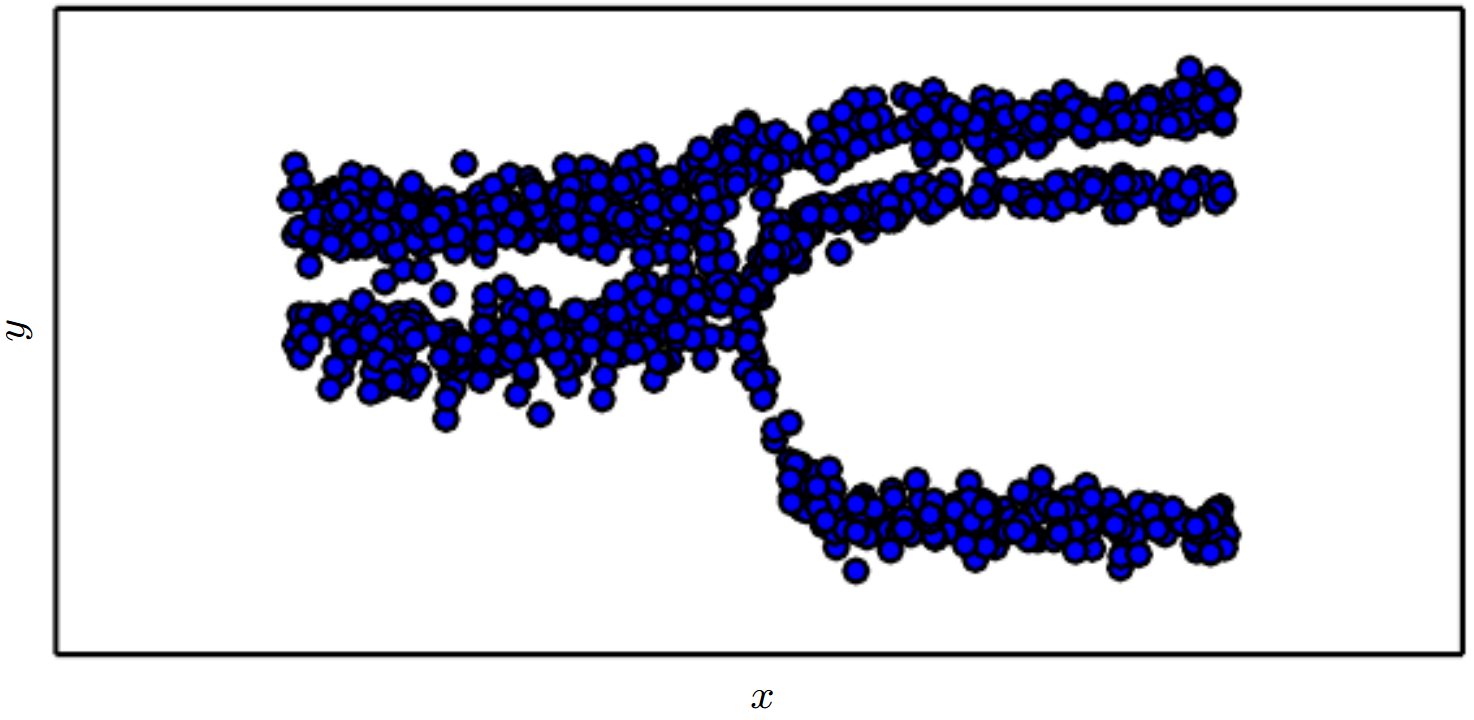
\includegraphics[width=0.8\textwidth]{FIG/fig6_4.PNG}
        \caption{Samples drawn from a neural network with a mixture density output layer.
          The input $x$ is sampled from a uniform distribution,
          and the output $y$ is sampled from $p _ {model} (y\ |\ x)$.
          The neural network is able to learn nonlinear mappings from the input to the parameters of the output distribution.
          These parameters include the probabilities governing which of three mixture components will generate the output as well as the parameters for each mixture component.
          Each mixture component is Gaussian with predicted mean and variance.
          All these aspects of the output distribution are able to vary with respect to the input $x$,
          and to do so in nonlinear ways.
        }\label{fig:NN_mixture_density_output_layer}
      \end{center}
    \end{figure}

    Figure~\ref{fig:NN_mixture_density_output_layer} is an example of mixture density network.

  \end{itemize}


\section{Ch10.9 Leaky Units and Other Strategies for Multiple Time Scales}
\label{Ch10.9}
\input{Ch10.9}
\section{Ch20.1 Boltzmann Machines}
\label{Ch20.1}
\input{Ch20.1}
\end{document}
